\documentclass[a4paper,11pt]{kth-mag}
\usepackage[T1]{fontenc}
\usepackage{textcomp}
\usepackage{lmodern}
\usepackage{datetime}
\usepackage[utf8]{inputenc}
\usepackage[swedish,english]{babel}
\usepackage{modifications}
\usepackage{graphicx}
\selectlanguage{swedish}
\title{Benchmarking Human Solving Methods for
           Rubik's cube}

\subtitle{Duis autem vel eum iruire dolor in hendrerit in
          vulputate velit esse molestie consequat, vel illum
          dolore eu feugiat null}
\foreigntitle{Sammanfattning}
\author{Andreas Nilsson  anil9@kth.se\\Anton Spång  aspang@kth.se}
\date{\today}

\blurb{DD143X - Bachelor Thesis\\Supervisor: Michael Schliephake\\Examiner: Örjan Ekeberg}
\trita{TRITA xxx yyyy-nn}
\begin{document}
\frontmatter
\pagestyle{empty}
\removepagenumbers
\maketitle
\selectlanguage{english}
\begin{abstract}
  This is a skeleton for KTH theses. More documentation
  regarding the KTH thesis class file can be found in
  the package documentation.


\end{abstract}
\clearpage
\begin{foreignabstract}{swedish}
  Denna fil ger ett avhandlingsskelett.
  Mer information om \LaTeX-mallen finns i
  dokumentationen till paketet.


\end{foreignabstract}
\clearpage
\tableofcontents*
\mainmatter
\pagestyle{newchap}
\chapter{Introduction}
\begin{figure}[b!]
	
	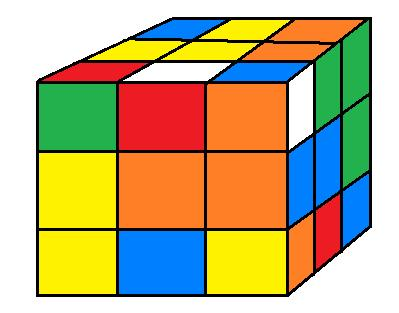
\includegraphics[width=0.5\textwidth]{scramble.jpg}
	\caption{Scrambled cube}
\end{figure}
\section{Problem Definition}
\section{Problem Statement}
\section{Purpose}
\section{Structure}

\chapter{Background}
\section{Competitions}
\subsection{Speedcubing}
\subsection{Fewest moves}
\section{Rubik's Cube}
\subsection{Description}
\subsection{Notation}
\section{Algorithms}
\subsection{Lbl using daisy method}
\subsubsection{White cross}
\subsubsection{White corners}
\subsubsection{Middle layer edges}
\subsubsection{Yellow cross}
\subsubsection{Yellow corners}
\subsubsection{Last layer permutation}
\subsection{Dedmore algorithm}
\subsubsection{Top corners (the X)}
\subsubsection{Top edges}
\subsubsection{Middle layer}
\subsubsection{Bottom corners}
\subsubsection{Bottom edges}

\chapter{Method}

\section{Literature study}
\section{Implementation and data collection}
\section{Analyze and representation}


\chapter{Implementation}
\section{Cube representation}
\section{Algorithms}
\section{Scramble}
\section{Difficulty}

\chapter{Results and Analyze}

\section{Data}
\section{Comparison}

\chapter{Discussion}

\section{Comparison}
\section{Errors}

\chapter{Conclusion}
\cite{MadeHow}
\renewcommand{\bibname}{References}
\bibliographystyle{plain}
\bibliography{references}

\appendix
\addappheadtotoc
\chapter{RDF}\label{appA}

\begin{figure}[ht]
\begin{center}
And here is a figure
\caption{\small{Several statements describing the same resource.}}\label{RDF_4}
\end{center}
\end{figure}

that we refer to here: \ref{RDF_4}
\end{document}
